% BEGIN TEMPLATE
\documentclass{article}
\usepackage{graphicx}
\usepackage{hyperref} 
\usepackage{xcolor}
\usepackage{nameref}
\usepackage{listings}
\usepackage{float}
\usepackage[title]{appendix}
\usepackage[ruled]{algorithm2e}
\graphicspath{ {../../images/} }
\bibliographystyle{acm}
% CHANGE THESE
\newcommand{\courseListing}{CSCI 8920}
\newcommand{\courseName}{Fundamentals of Deep Learning}
\newcommand{\assignmentTitle}{Homework Assignment \#4}
\newcommand{\assignmentSubtitle}{Attention Modules: CBAM}
\usepackage{geometry}
\geometry{margin=1in}

\hypersetup{
    colorlinks,
    linkcolor={red!50!black},
    citecolor={blue!50!black},
    urlcolor={blue!80!black}
}
\urlstyle{same}
\definecolor{codegreen}{rgb}{0,0.6,0}
\definecolor{codegray}{rgb}{0.5,0.5,0.5}
\definecolor{codepurple}{rgb}{0.58,0,0.82}
\lstdefinestyle{mystyle}{
    commentstyle=\color{codegreen},
    keywordstyle=\color{magenta},
    numberstyle=\tiny\color{codegray},
    stringstyle=\color{codepurple},
    basicstyle=\ttfamily\footnotesize,
    breakatwhitespace=false,         
    breaklines=true,                 
    captionpos=b,                    
    keepspaces=true,                 
    numbers=left,                    
    numbersep=5pt,                  
    showspaces=false,                
    showstringspaces=false,
    showtabs=false,                  
    tabsize=2
}

\lstset{style=mystyle}

\begin{document}
  \begin{center}
  
\includegraphics[scale=0.15]{UNO-Logo-Color.png}
  \\[0.3in]
  \textbf{\courseListing{}}\\
  \courseName{}
  \\[0.75in]
  \textbf{\assignmentTitle{}}\\
  \assignmentSubtitle{}
  \\[0.75in]
  \textbf{Patrick Davlin}
  \\[0.75in]
  \textbf{Computer Science Department}\\
  \textbf{Peter Kiewit Institute}\\
  \textbf{University of Nebraska}
  \\[0.75in]
  \textbf{Spring 2021}
  \\[0.3in]
  
\includegraphics[scale=0.075]{UNO-Icon-Color.png}
  \newpage
\end{center}
  \graphicspath{{./images/}}
% END TEMPLATE

\section{Project Setup} \label{setup}
Similarly to past work in this course, this assignment was done entirely on a local machine using the following specific packages:
\begin{itemize}
    \item Python 3.8.6 
    \item Tensorflow 2.4.1
    \item Matplotlib 3.3.4
\end{itemize}.

There is little else to say about the setup. With the Tensorflow tooling configured there is relatively little variation from assignment to assignment. 

In terms of the assignment itself, it is worth noting that similar work was completed last semester as part of the CSCI 8110 course.
In an attempt to extend the learning from that project, CBAM was implemented for this assignment, in hopes that some comparisons might be possible between the two attention modules.
The CSCI 8110 assignment document can be found \href{https://keybase.pub/pdav/academics/8110\%20Reports/Davlin_HW3_V2.pdf}{via the hyperlink on this text}.

\section{Implementation} \label{impl}
\textit{Note: this section discusses sections of code; the entire project can be found in the \nameref{codelist}}.

The first task in this assignment was gaining an understanding of the CBAM attention module and its structure.
The CBAM module, fundamentally, is composed of two parts--the \textit{Channel Attention Module} and the \textit{Spatial Attention Module}.
These two submodules focus, according to the original paper's authors, on the "what" and the "where," respectively, for identifying an image.
For best results, they note, placing the modules sequentially is an optimal approach.
With that in mind, a graphical representation of the CBAM module structure looks like the following: 

\begin{figure}[H]
    \centering
    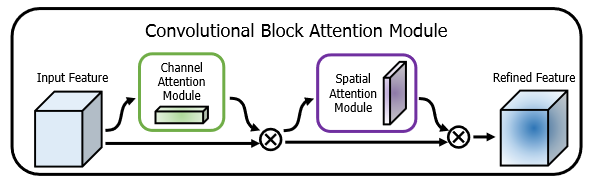
\includegraphics[width=5in]{csci-8920/hw-4/images/cbam-full-diagram.png}
    \caption{CBAM full module diagram. \textit{Source: Woo, et al.} \cite{Woo2018CBAM:Module}}
    \label{fig:cbam_full_diag}
\end{figure}

The independent submodules can also be broken down, as follows:

\begin{figure}[H]
    \centering
    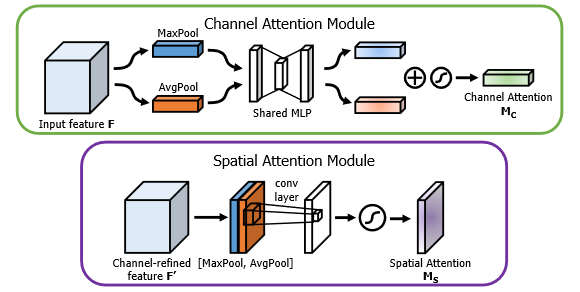
\includegraphics[width=5in]{csci-8920/hw-4/images/cbam-module-diagrams.png}
    \caption{CBAM submodule diagram. \textit{Source: Woo, et al.} \cite{Woo2018CBAM:Module}}
    \label{fig:cbam_mod_diag}
\end{figure}

Using these figures as a road map of sorts, constructing the complete CBAM model was possible.
One interesting aspect of the CBAM architecture is that the \lstinline{MaxPool} and \lstinline{AvgPool} operations are performed independently and then combined afterwards in the Channel Attention Module.
This particular approach was novel, at least in the scope of prior homework projects, and can be observed below:

\begin{lstlisting}[language=Python]
def channel_attention(input_feature, ratio=8):
    channel_axis = 1 if K.image_data_format() == "channels_first" else -1
    channel = input_feature.shape[channel_axis]

    avg_pool = GlobalAveragePooling2D()(input_feature)
    avg_pool = Reshape((1,1,channel))(avg_pool)
    avg_pool = Dense(channel//ratio, activation='relu', kernel_initializer='he_normal', use_bias=True, bias_initializer='zeros')(avg_pool)
    avg_pool = Dense(channel, kernel_initializer='he_normal', use_bias=True, bias_initializer='zeros')(avg_pool)

    max_pool = GlobalMaxPooling2D()(input_feature)
    max_pool = Reshape((1,1,channel))(max_pool)

    max_pool = Dense(channel//ratio, activation='relu', kernel_initializer='he_normal', use_bias=True, bias_initializer='zeros')(max_pool)
    max_pool = Dense(channel, kernel_initializer='he_normal', use_bias=True, bias_initializer='zeros')(max_pool)

    combined = Add()([avg_pool, max_pool])
    combined = Activation('sigmoid')(combined)

    if K.image_data_format == "channels_first":
        combined = Permute((3,1,2))(combined)

    return multiply([input_feature, combined]) 
\end{lstlisting}

The Spatial Attention Module has a similar piecewise implementation of the max and average pooling, using \lstinline{Lambda()} layers:

\begin{lstlisting}[language=Python]
def spatial_attention(input_feature, kernel_size=7):
    if K.image_data_format() == "channels_first":
        channel = input_feature.shape[1]
        cbam_feature = Permute((2,3,1))(input_feature)
    else:
        channel = input_feature.shape[-1]
        cbam_feature = input_feature

    avg_pool = Lambda(lambda x: K.mean(x, axis=3, keepdims=True))(cbam_feature)
    max_pool = Lambda(lambda x: K.max(x, axis=3, keepdims=True))(cbam_feature)

    combined = Concatenate(axis=3)([avg_pool, max_pool])

    cbam_feature = Conv2D(filters = 1, kernel_size = kernel_size, strides=1, padding='same', activation='sigmoid', kernel_initializer='he_normal', use_bias=False)(combined)

    if K.image_data_format() == "channels_first":
        cbam_feature = Permute((3, 1, 2))(cbam_feature)

    return multiply([input_feature, cbam_feature])
\end{lstlisting}

With these modules created, and combined sequentially in a separate function, it was a fairly simple exercise to extend an existing VGG16 model to include them after each of several "checkpoints."
The complete CBAM module needed to be included after each of several layers in VGG16:
\begin{itemize}
    \item between input and conv 1-1;
    \item between pooling and conv 2-1; 
    \item between pooling and conv 3-1;  
    \item between pooling and conv 4-1;  
    \item between pooling and 5-1; 
    \item between pooling and dense
\end{itemize}

This implementation was completed as follows, where layer numbers indicate each of the desired checkpoints.
Also note that a new softmax layer was substituted at the end to reduce the number of considered categories to ten, for purposes of training against the imagenette dataset.
After compilation, the model is trained against that dataset and saved for later use.
The basic concept of this code was pulled directly from the prior semester's assignment.

\begin{lstlisting}[language=Python]
for layer_loc in [3,6,10,14,18]:
  # copy off the original model so we can compare later
  model_copy = model

  for il in range(len(model_copy.layers) - 1):
    if il == 0:
      xl = model_copy.layers[il].output
    else:
      xl = model_copy.layers[il](xl)
    # locations of pooling: 3,6,10,14,18
    # can change location accordingly
    if il == layer_loc:
      xl = CBAM_impl(xl)

  # reduced softmax layer (to reduce number of considered categories to 10)
  xl = Dense(10,activation='softmax')(xl)

  # define new model with CBAM block
  new_model= Model(model_copy.input,xl)

  # compile new model
  new_model.compile(
    optimizer='adam',
    loss='sparse_categorical_crossentropy',
    metrics=['accuracy']
  )
  
    new_model.fit(training_dataset,
                validation_data=validation_dataset,
                batch_size=128,
                epochs=10)
  
  new_model.save('./models/cbam-layer-{}'.format(layer_loc))
\end{lstlisting}

Finally, each resulting model is pulled from a saved folder and plotted.
An arbitrary image was selected from the imagenette dataset for demonstration purposes:

\begin{figure}[H]
    \centering
    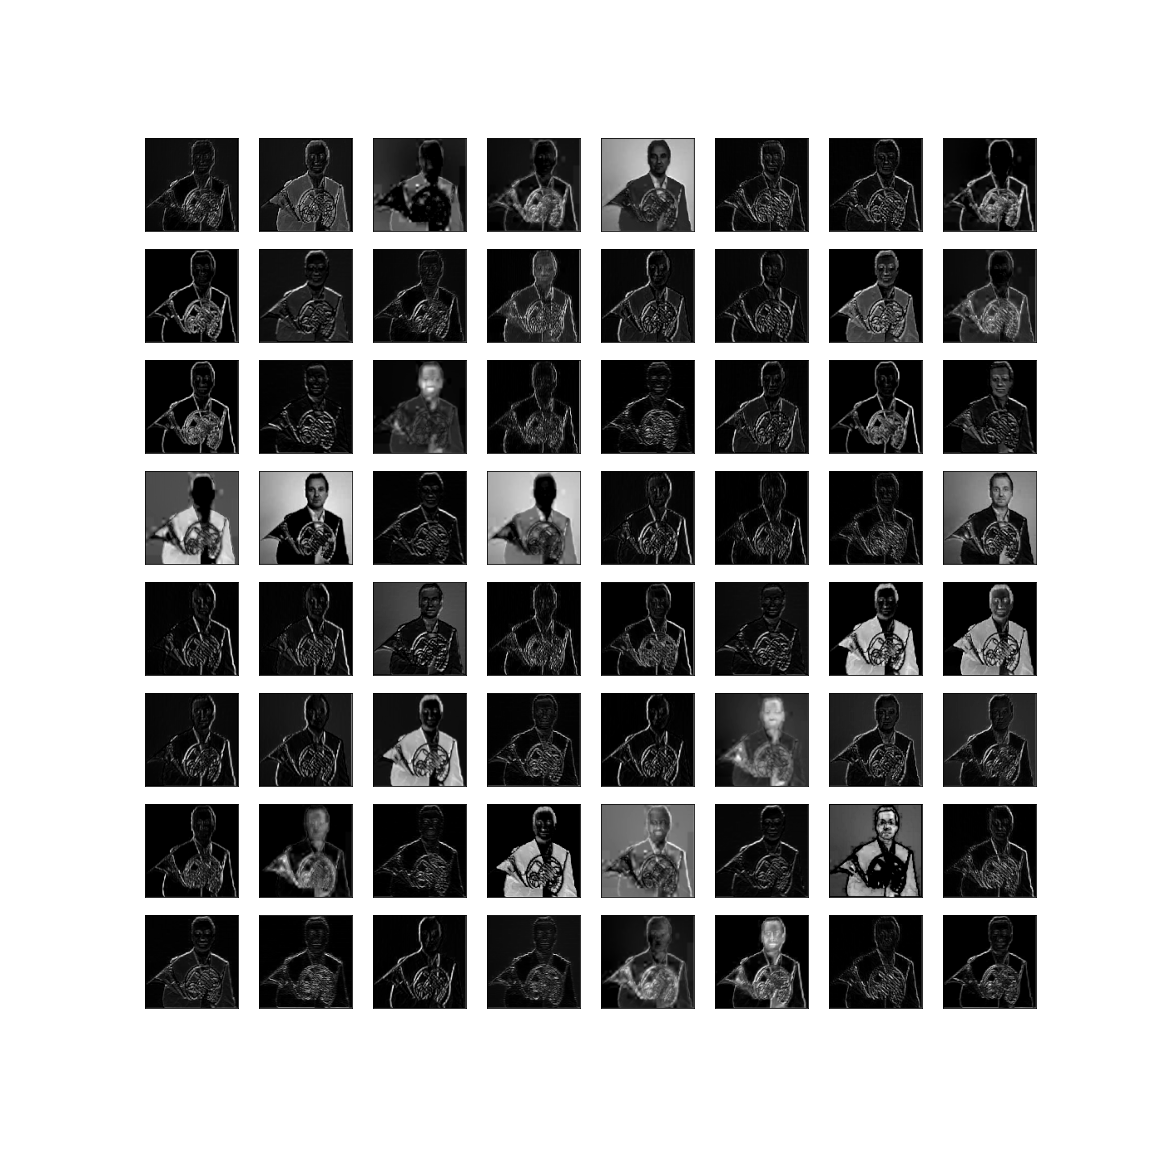
\includegraphics[width=6in]{csci-8920/hw-4/images/horn-pre-CBAM-3-block1_pool.png}
    \caption{French horn feature map after \lstinline{block1_pool}, before CBAM}
    \label{fig:horn_1_pre}
\end{figure}

\begin{figure}[H]
    \centering
    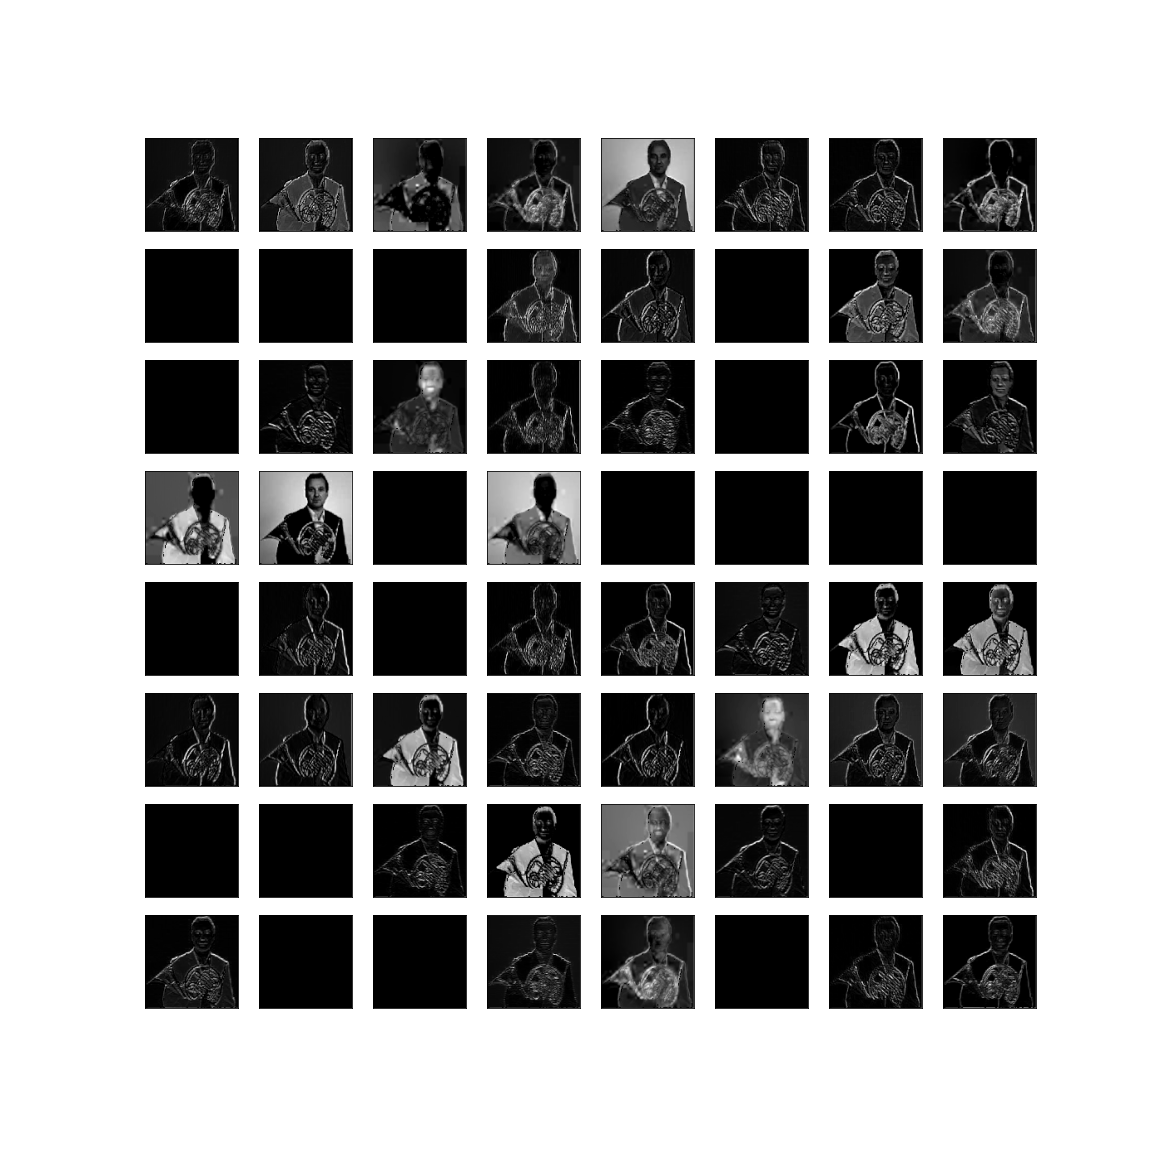
\includegraphics[width=6in]{csci-8920/hw-4/images/horn-post-CBAM-3-block1_pool.png}
    \caption{French horn feature map after \lstinline{block1_pool}, after CBAM}
    \label{fig:horn_1_post}
\end{figure}

More outputs can be found in the \nameref{outputlist} Appendix.

\section{Conclusions}
While not altogether new, as a student continuing in the deep learning coursework pipeline from CSCI 8110, the implementation of CBAM in CSCI 8920 has been an interesting and enlightening experience.
One area of note from last semester is that the code used to implement CBAM now is generally more efficient; no doubt a benefit of the "second look" taken from the previous code.
The CBAM module itself is similar in concept to the SENet, but it was interesting to see the ways in which the CBAM approach is different.
Observing the series of graphs output from the module provides a lot of insight into how the VGG16 model "hones in" on the elements of the French horn image, and with other imagenette images.


\bibliographystyle{unsrt}
\bibliography{references}

\newpage
\begin{appendices}
\section{Complete Model Output Listing} \label{outputlist}

\begin{figure}[H]
    \centering
    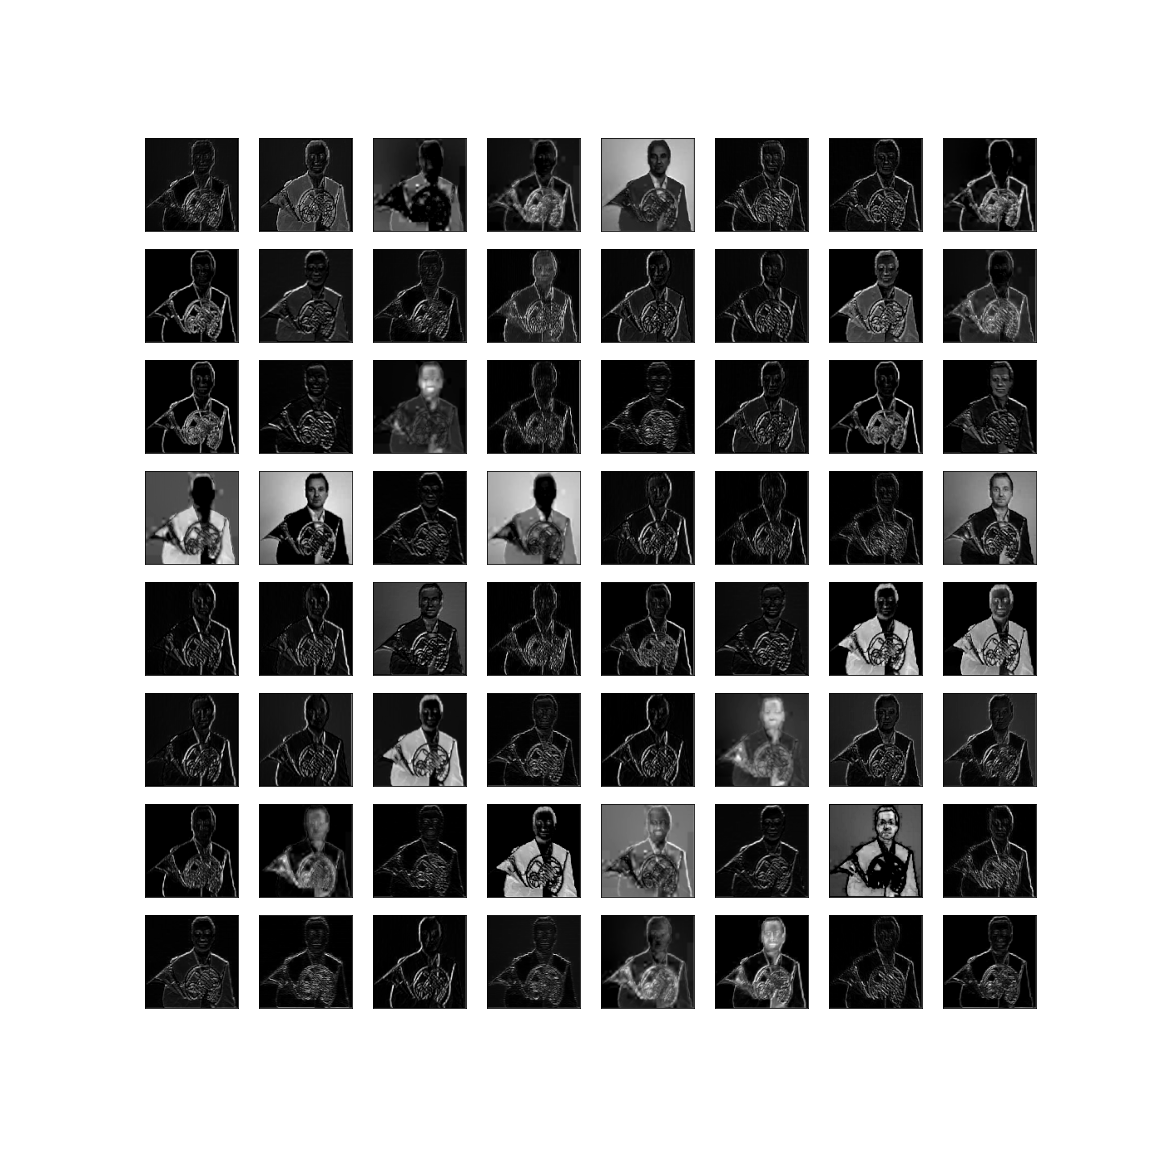
\includegraphics[width=3in]{csci-8920/hw-4/images/horn-pre-CBAM-3-block1_pool.png}
    \caption{French horn feature map after \lstinline{block1_pool}, before CBAM}
    \label{fig:horn_2_pre}
\end{figure}

\begin{figure}[H]
    \centering
    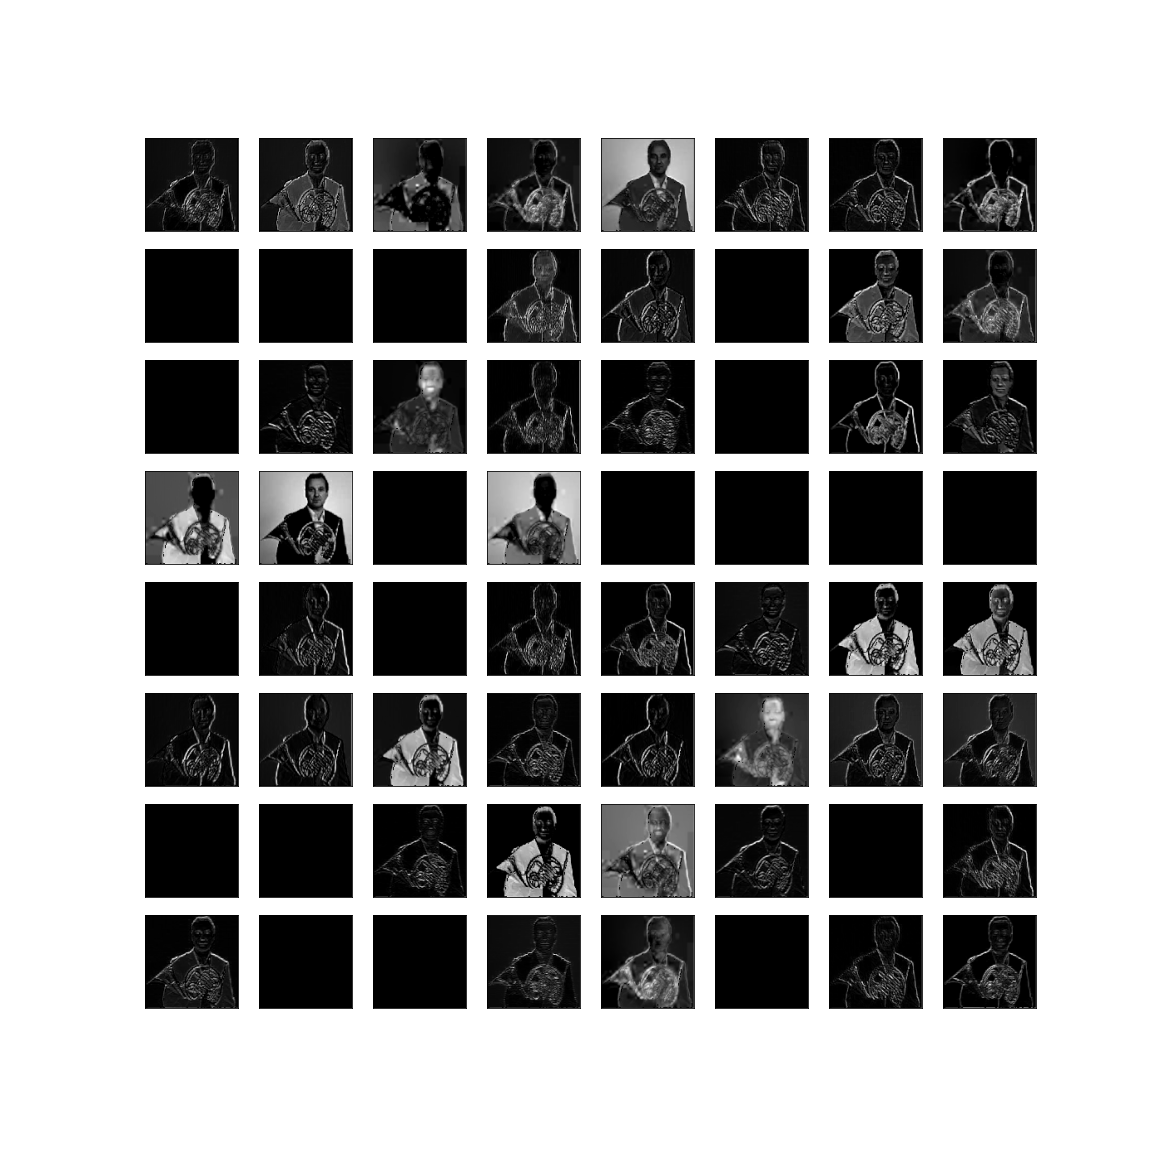
\includegraphics[width=3in]{csci-8920/hw-4/images/horn-post-CBAM-3-block1_pool.png}
    \caption{French horn feature map after \lstinline{block1_pool}, after CBAM}
    \label{fig:horn_2_pre}
\end{figure}

\begin{figure}[H]
    \centering
    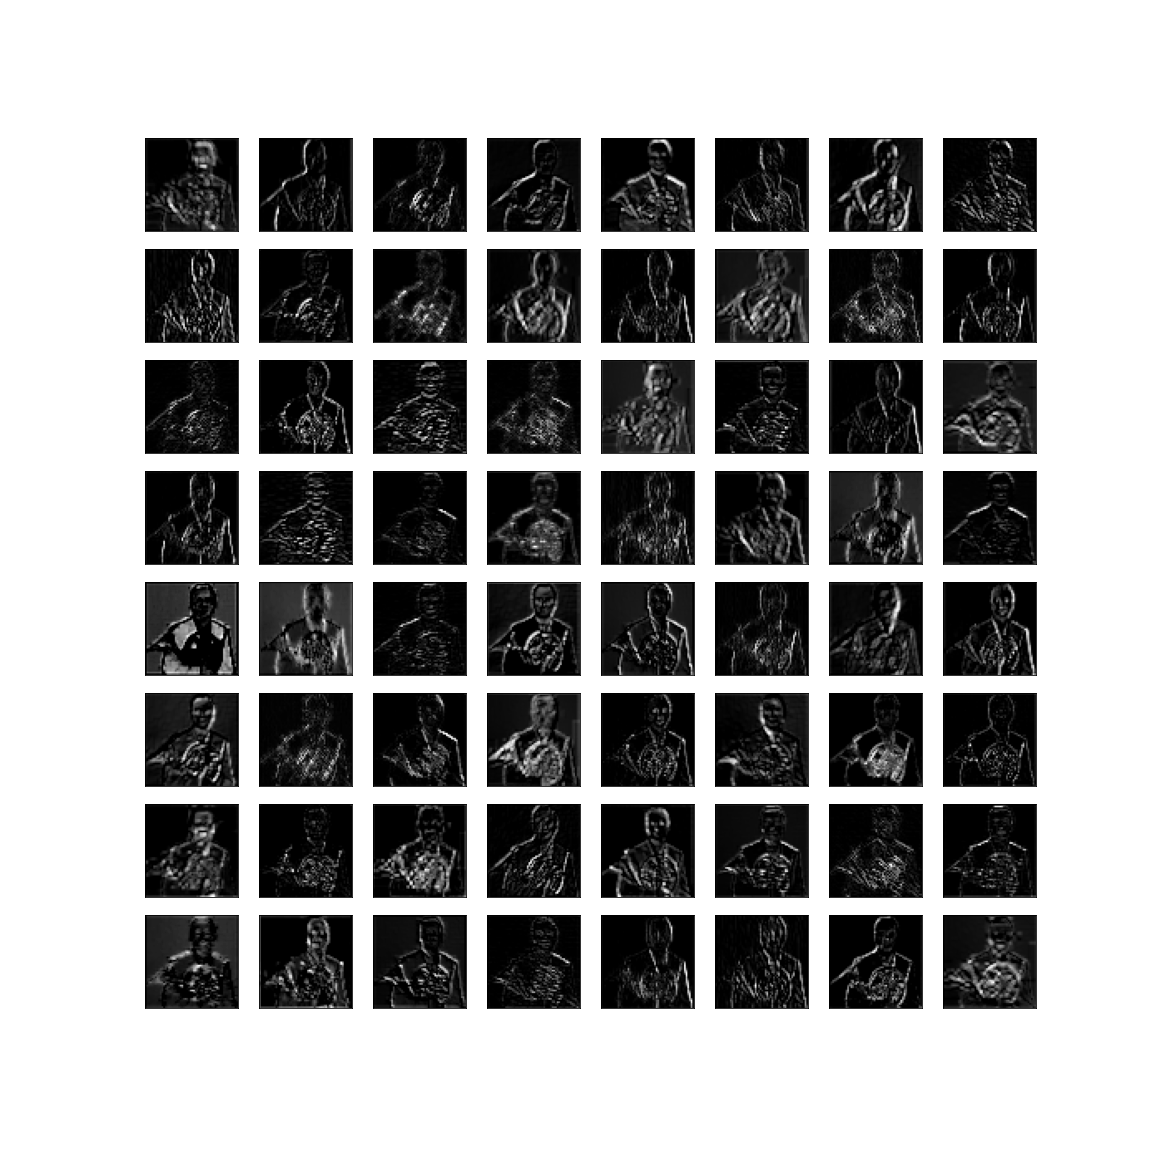
\includegraphics[width=3in]{csci-8920/hw-4/images/horn-pre-CBAM-6-block2_pool.png}
    \caption{French horn feature map after \lstinline{block2_pool}, before CBAM}
    \label{fig:horn_2_post}
\end{figure}
\begin{figure}[H]
    \centering
    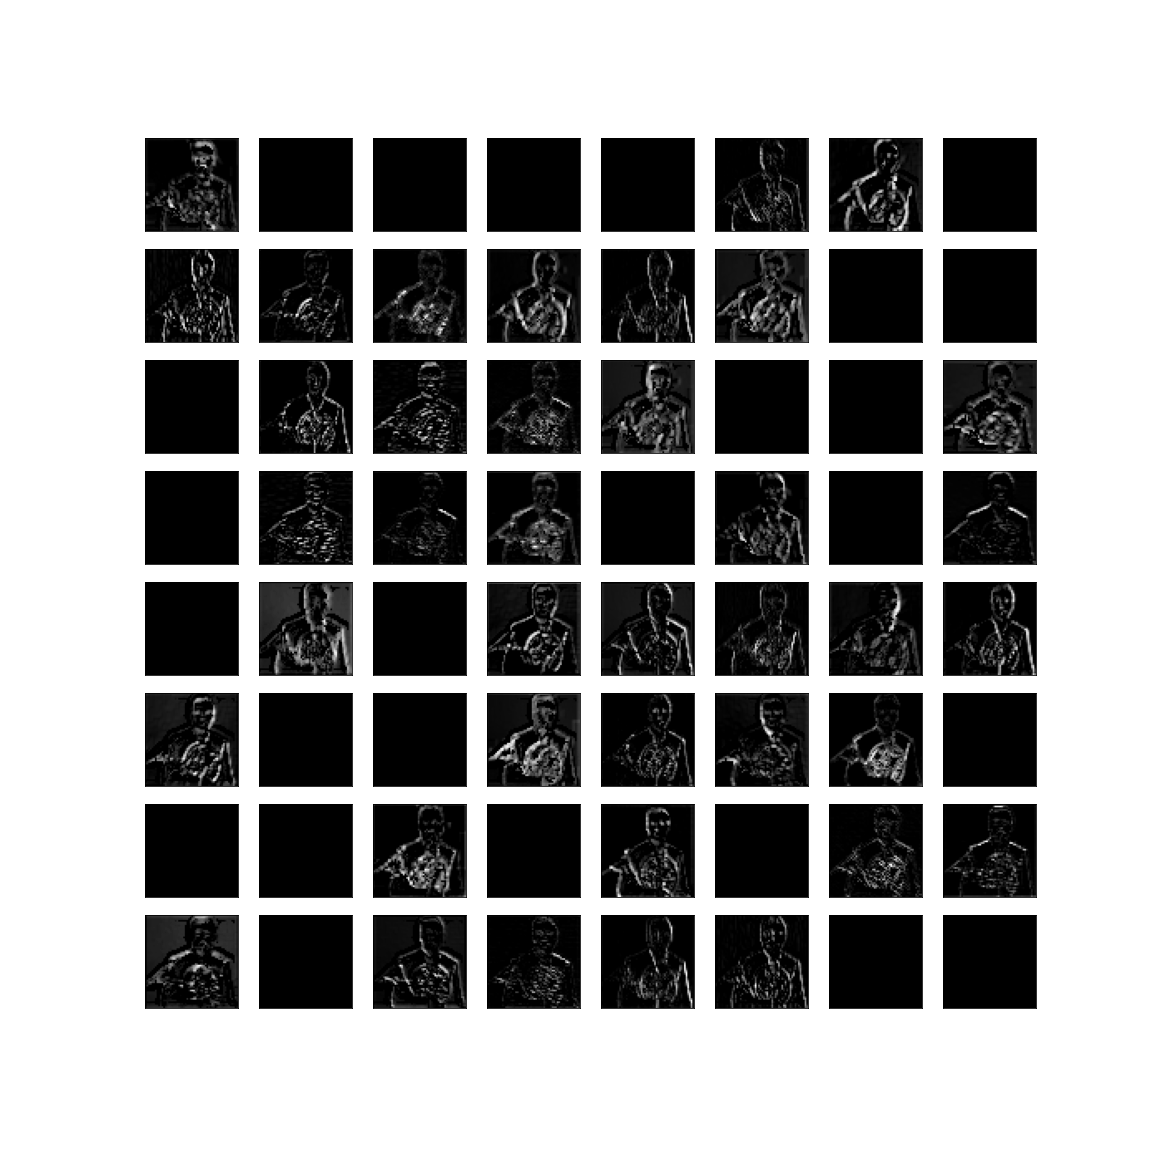
\includegraphics[width=3in]{csci-8920/hw-4/images/horn-post-CBAM-6-block2_pool.png}
    \caption{French horn feature map after \lstinline{block2_pool}, after CBAM}
    \label{fig:horn_3_pre}
\end{figure}

\begin{figure}[H]
    \centering
    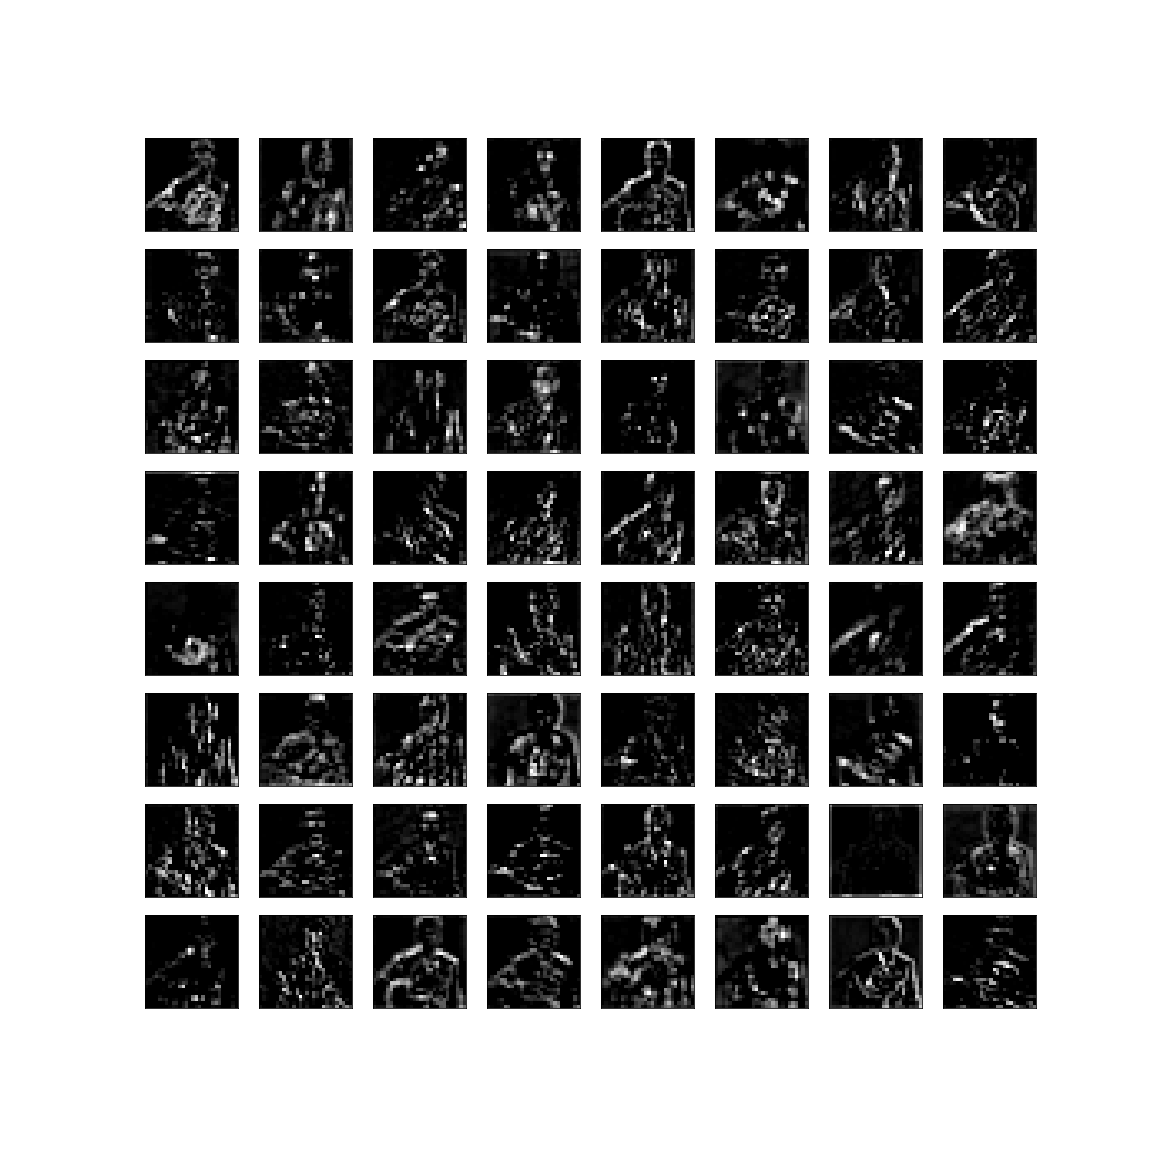
\includegraphics[width=3in]{csci-8920/hw-4/images/horn-pre-CBAM-10-block3_pool.png}
    \caption{French horn feature map after \lstinline{block3_pool}, before CBAM}
    \label{fig:horn_3_post}
\end{figure}
\begin{figure}[H]
    \centering
    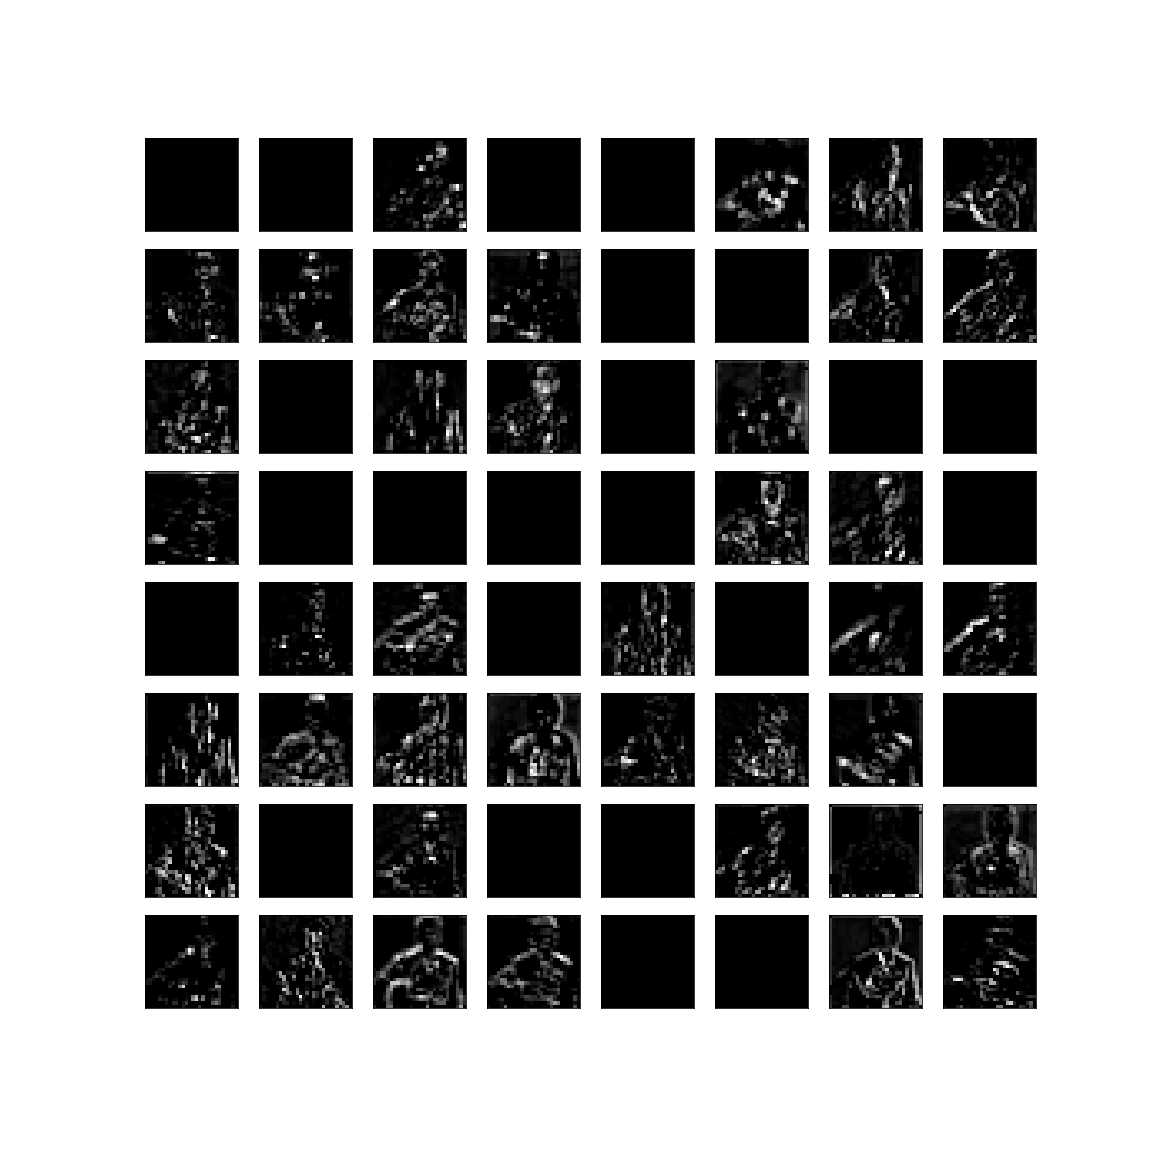
\includegraphics[width=3in]{csci-8920/hw-4/images/horn-post-CBAM-10-block3_pool.png}
    \caption{French horn feature map after \lstinline{block3_pool}, after CBAM}
    \label{fig:horn_4_pre}
\end{figure}

\begin{figure}[H]
    \centering
    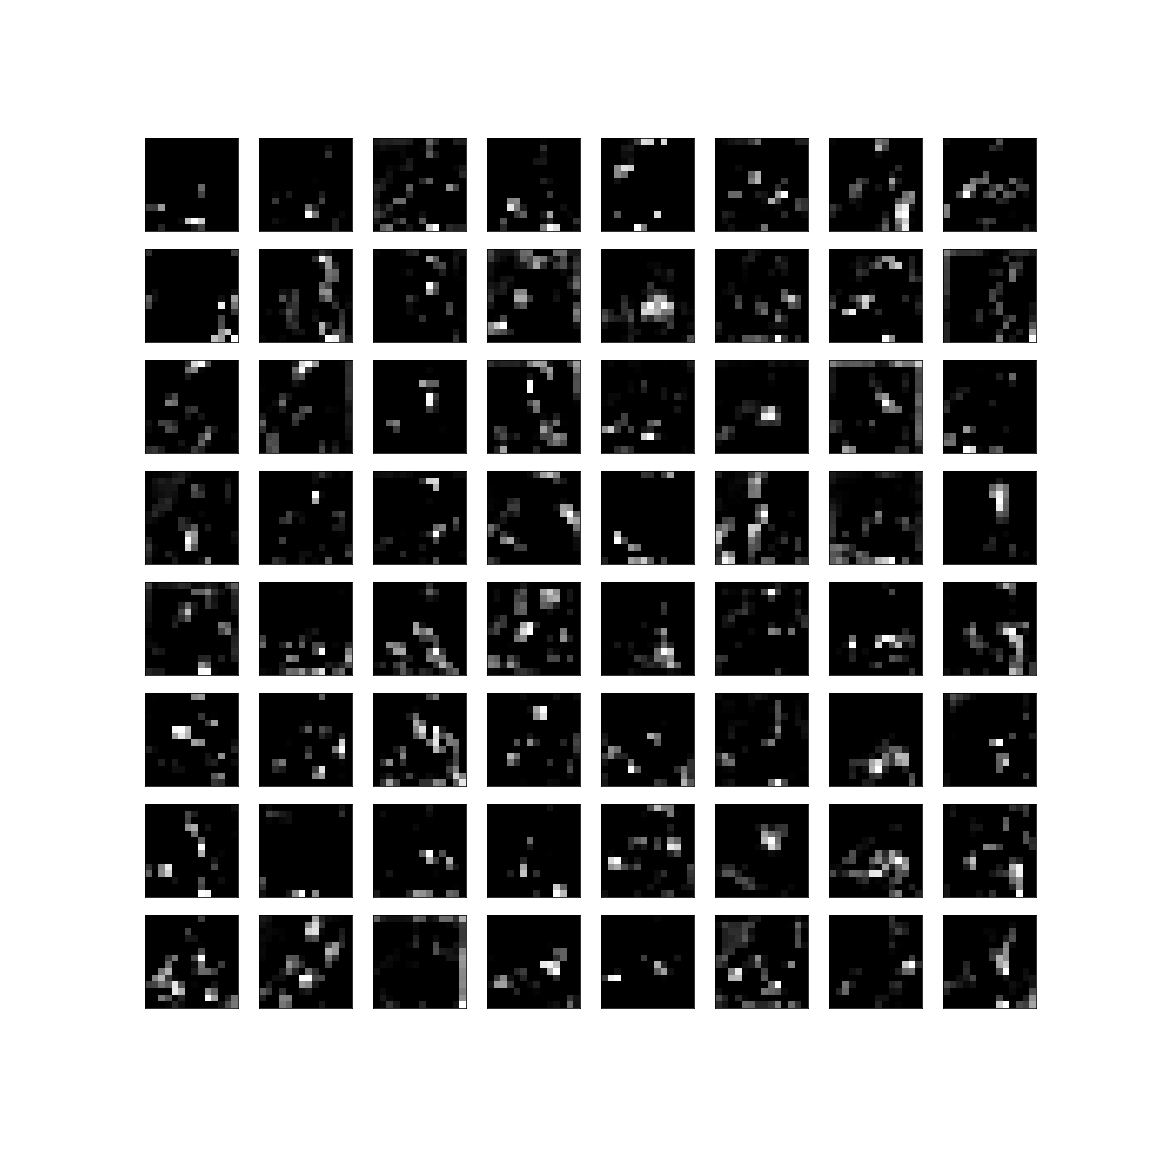
\includegraphics[width=3in]{csci-8920/hw-4/images/horn-pre-CBAM-14-block4_pool.png}
    \caption{French horn feature map after \lstinline{block4_pool}, before CBAM}
    \label{fig:horn_4_post}
\end{figure}
\begin{figure}[H]
    \centering
    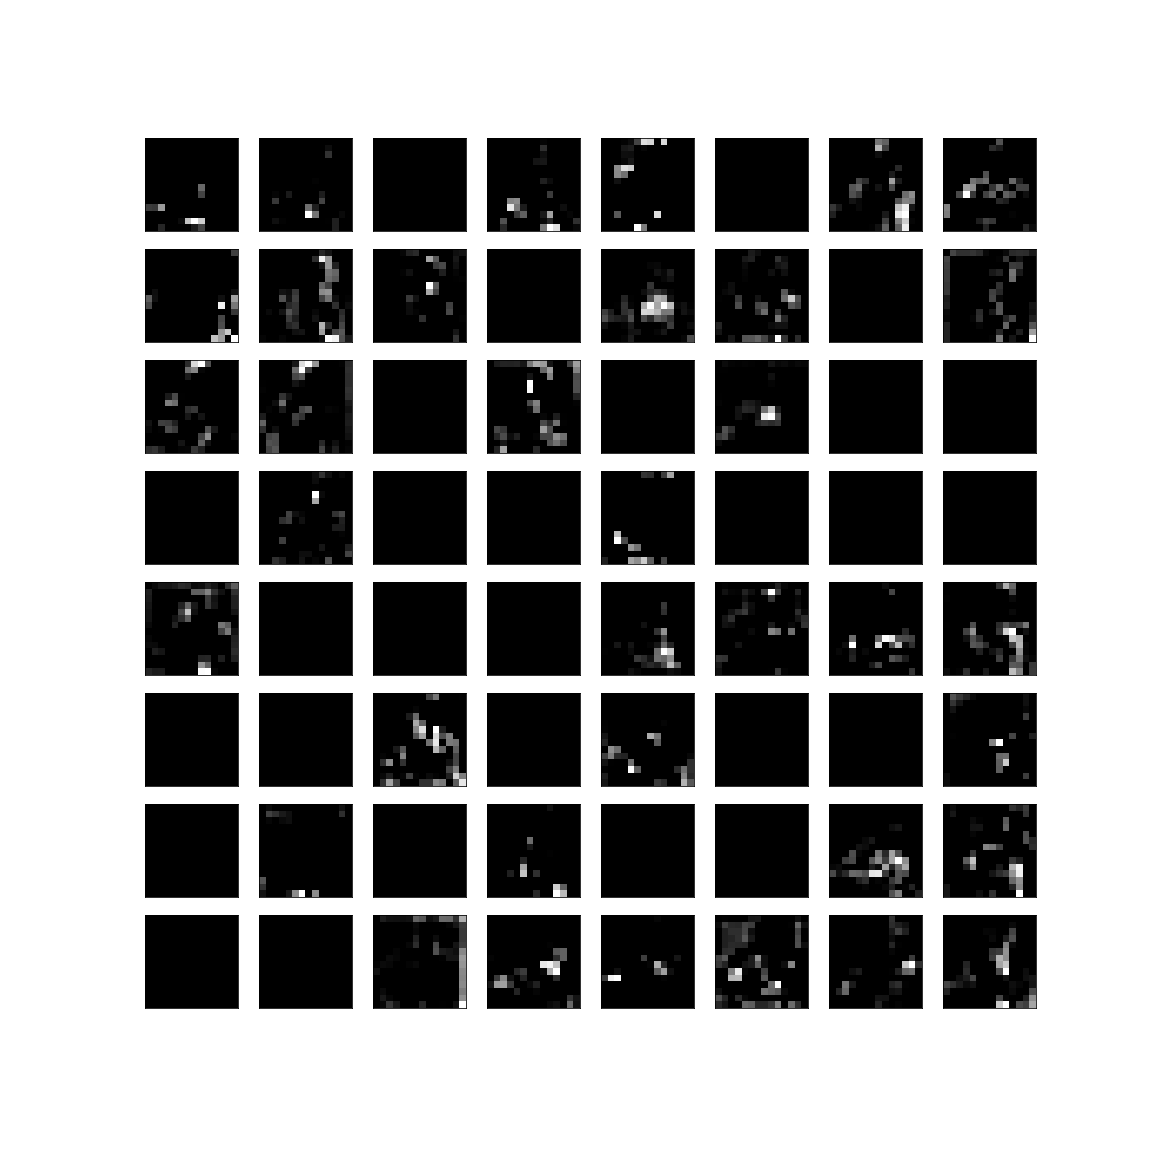
\includegraphics[width=3in]{csci-8920/hw-4/images/horn-post-CBAM-14-block4_pool.png}
    \caption{French horn feature map after \lstinline{block4_pool}, after CBAM}
    \label{fig:horn_5_pre}
\end{figure}

\begin{figure}[H]
    \centering
    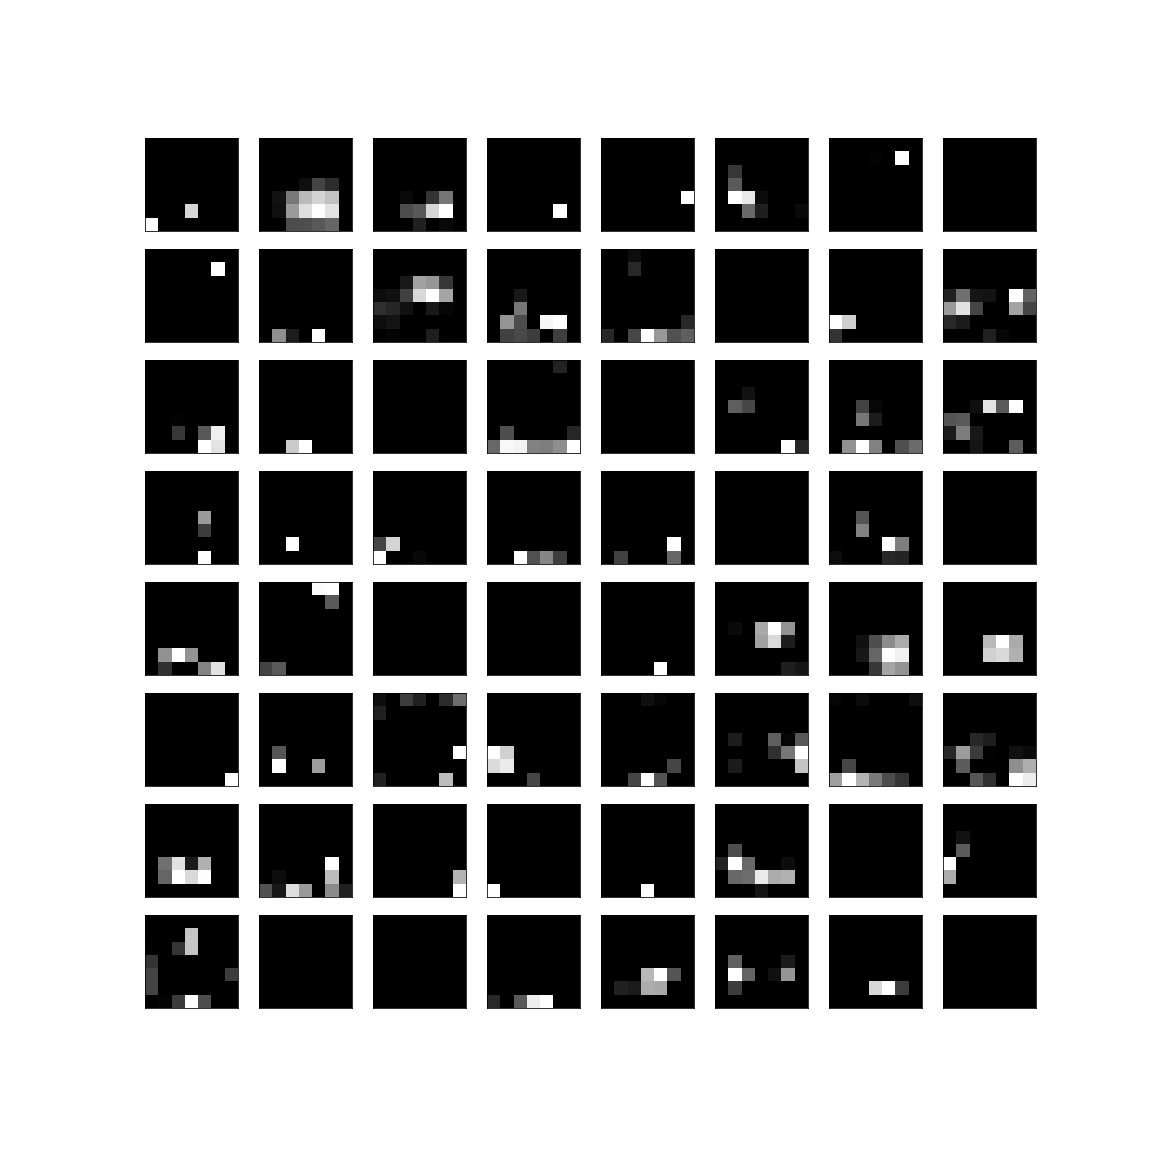
\includegraphics[width=3in]{csci-8920/hw-4/images/horn-pre-CBAM-18-block5_pool.png}
    \caption{French horn feature map after \lstinline{block5_pool}, before CBAM}
    \label{fig:horn_5_pre}
\end{figure}

\begin{figure}[H]
    \centering
    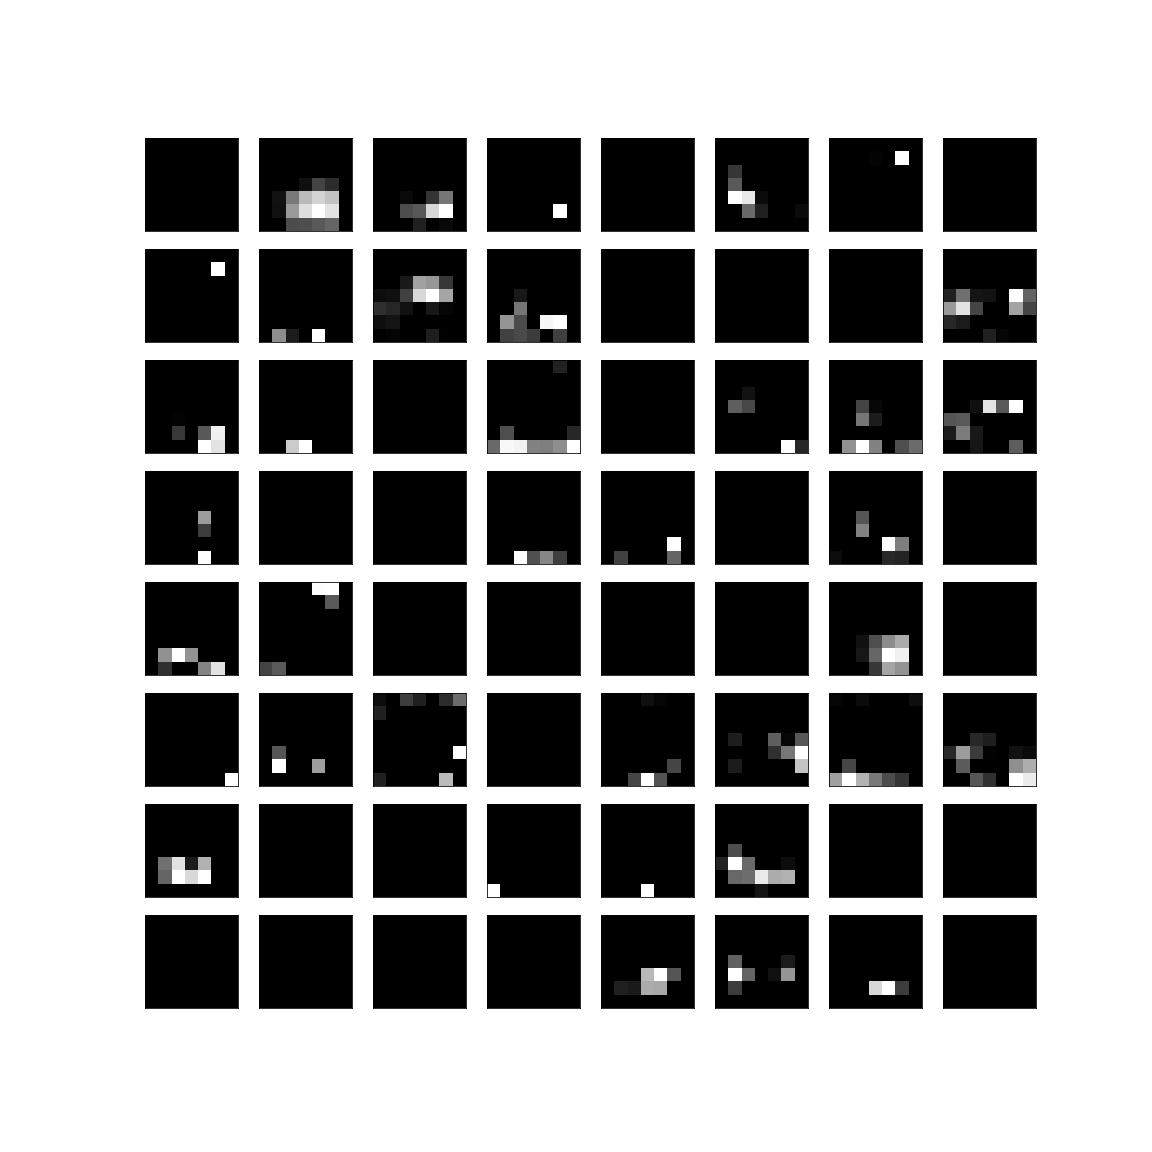
\includegraphics[width=3in]{csci-8920/hw-4/images/horn-post-CBAM-18-block5_pool.png}
    \caption{French horn feature map after \lstinline{block5_pool}, before CBAM}
    \label{fig:horn_5_post}
\end{figure}
\section{Complete Code Listing} \label{codelist}
\newpage
\lstinputlisting[language=Python]{hw-4.py}

\end{appendices}
\end{document}